% !TEX root = ../patchEmbeddings_review.tex

\section{Supplementary material}
\begin{itemize}
\item residual blocks with group normalization layers and skip-connections involving sum of feature maps from 
\item The input volume has shape $272 \times 272\times12$ which is equivalent to a volume of $544\times 544\times 12$ voxels in the original resolution $4\times 4\times 40$ nm$^3$. Before to apply the loss, we crop the predictions to a shape $224\times 224\times 9$ in order to avoid border artifacts. 
The final model trained on all available ground truth labels is trained with a slightly larger input volume of $288\times 288\times 14$ and we provide even more input to the cheaper glia-predictor-model: $352\times 352\times 15$ voxels. 
\item Explicitly say what is the size of the coarsest predicted mask in the original res, which should be $112 \times 112 \times 5$ voxels at res...
\item which outputs do we use for the averaging stuff? Only the high-res ones
\item Downscaled res
\item Crops in the decoder part, structure of the residual block
\item Adam Optimizer, learning rate, GroupNorm, residual blocks
\item Removing small segments
\item UNet: 3 depth levels with downscaling factor 2, feature maps, etc...
\item In the supplementary material, we provide all the architecture details: crops in the decoder of the UNet
\item we predict two types of \maskname masks at the highest level of the hierarchy
\end{itemize}

\textbf{Glia classifier} -- As a final post-processing step, we merge neighboring instances that have been classified as \emph{glia segments} (putative astrocyte). This is a common procedure in neuron segmentation \TODO{CIT}\cite{lee2019learning}, since glia segments are substantially different from the other neurons and are usually considered separately in the final reconstructed diagram of neural circuit connectivity. Glia segments usually present a main body with a lot of very thin glial processes


\begin{figure}[t]
\centering
        % \includegraphics[width=0.4\textwidth,trim=0.25in 0.25in 0.68in 0.36in,clip]{./figs/SSBM_experiments.pdf} % 0.45
        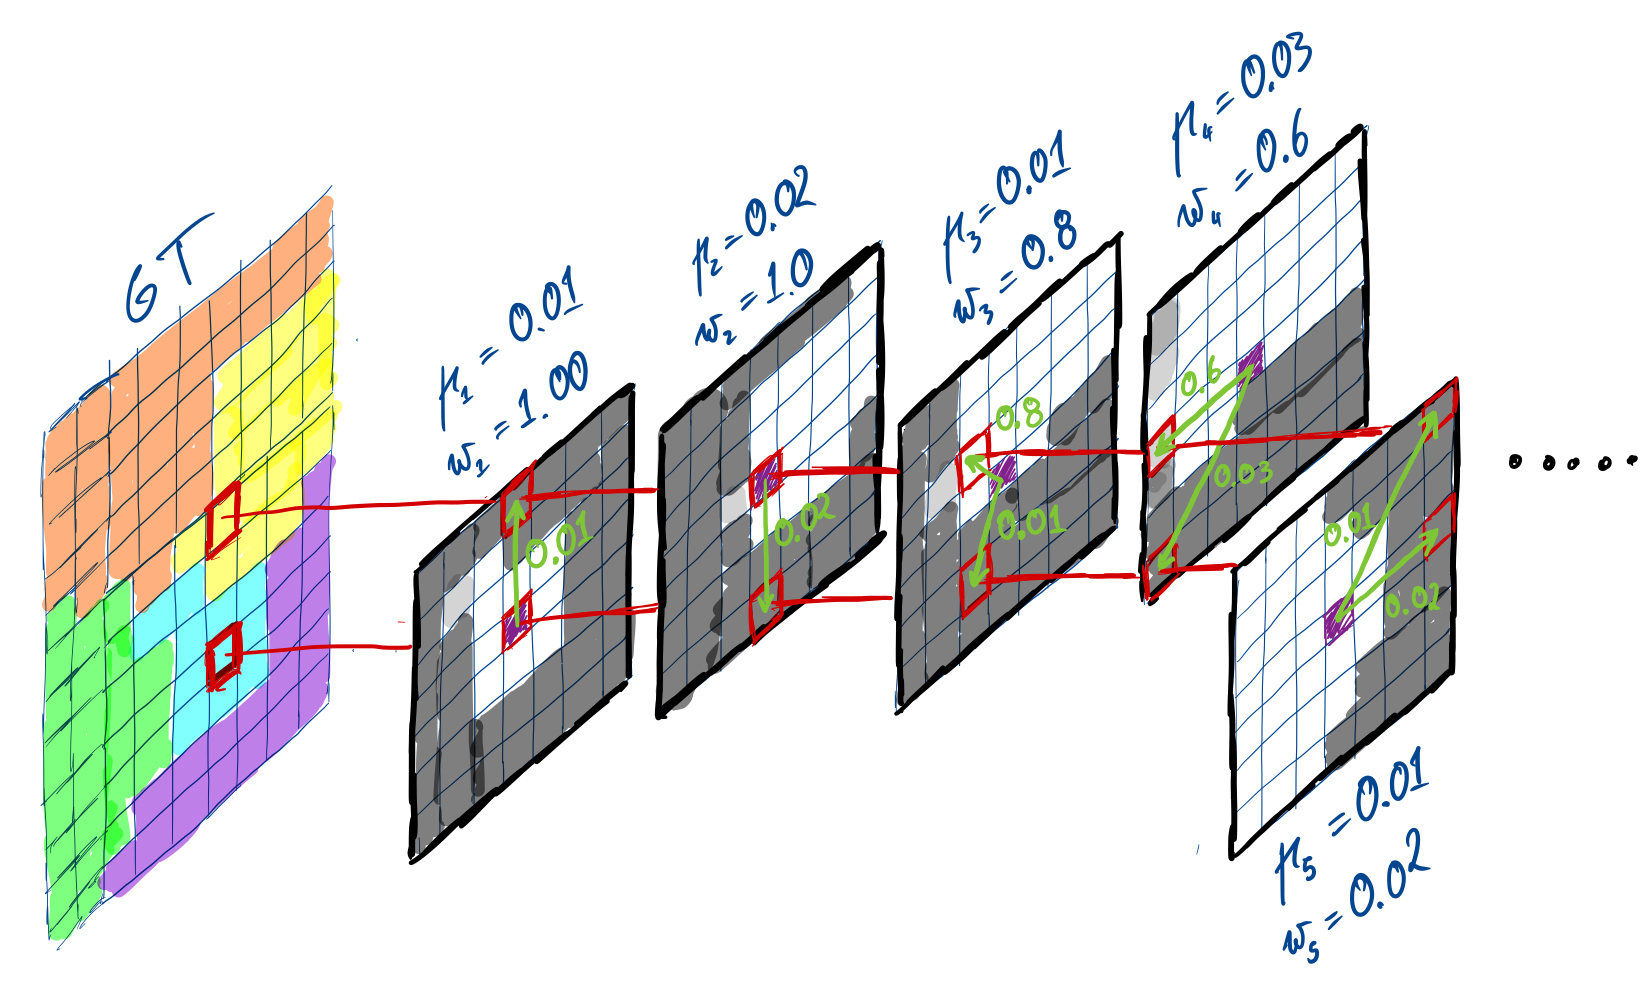
\includegraphics[width=0.7\textwidth]{./figs/alg_explaned.jpg} % 0.45
        \caption{\TODO{Update fig}  Illustration of the proposed parameter-free method to convert \maskname masks to edge weights...}
    \label{fig:alg_explained}
\end{figure}

\begin{figure}[t]
\centering
        % \includegraphics[width=0.4\textwidth,trim=0.25in 0.25in 0.68in 0.36in,clip]{./figs/SSBM_experiments.pdf} % 0.45
        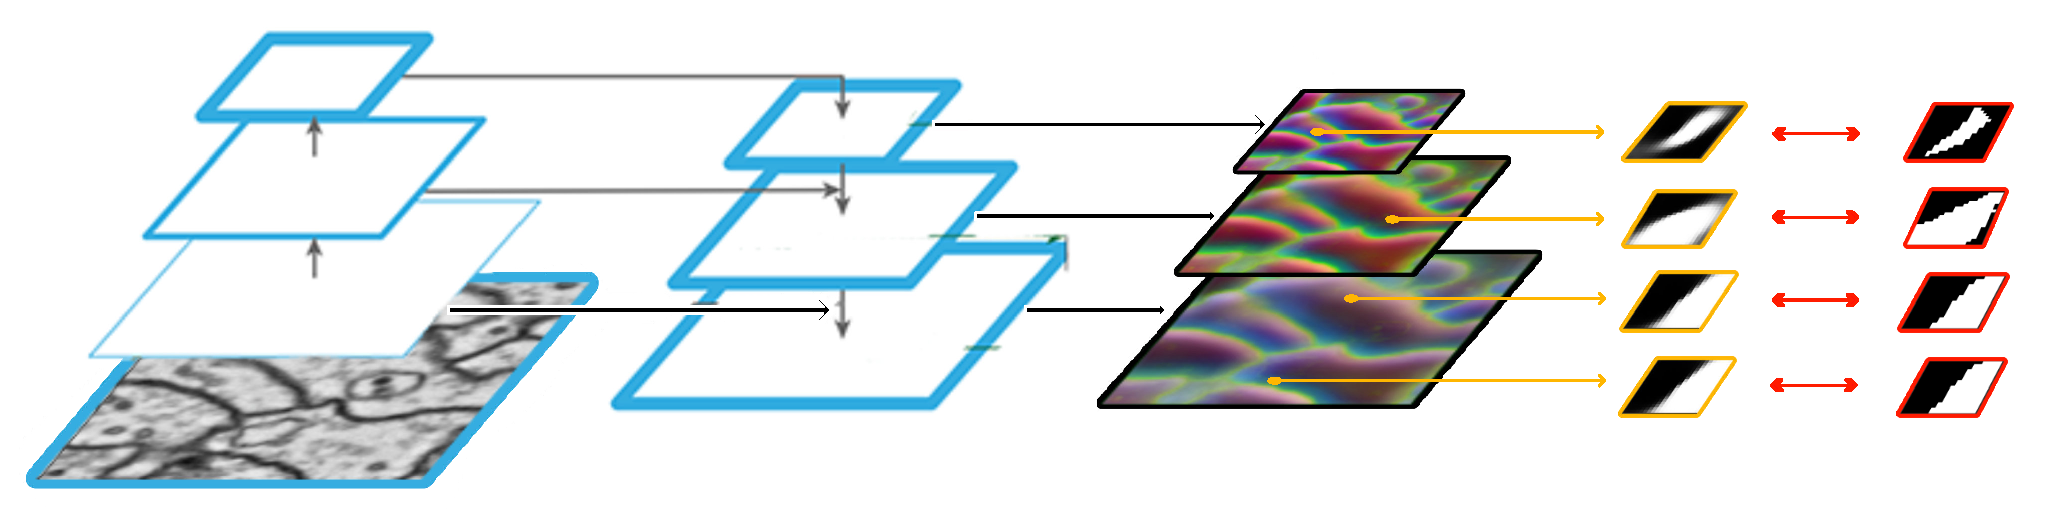
\includegraphics[width=\textwidth]{./figs/architecture.pdf} % 0.45
        \caption{\TODO{Update fig} Multi-scale patch prediction...}
    \label{fig:comparing_masks_affs}
\end{figure}

